\documentclass[10pt]{scrartcl} % use larger type; default would be 10pt

\usepackage[utf8]{inputenc} % set input encoding (not needed with XeLaTeX)
\usepackage[cm]{fullpage}
\usepackage{graphicx} % support the \includegraphics command and options
\usepackage{biblatex} % use biber command to regenerate references

\renewcommand{\bibfont}{\footnotesize}
%\pagenumbering{gobble}
\usepackage{hyperref}
\addbibresource{bib/proposal.bib}

\title{Accurate Vision-Based Landing For Multicopter UAVs}
\subtitle{CS287: Project Report}
\author{Constantin Berzan, Sunil Shah}
\date{} 

\begin{document}
\maketitle

\begin{abstract}
Multicopter UAVs have become increasingly popular over the last five years and are quickly becoming used for commercial purposes. However, they are hampered by their limited battery life. This class project is part of a larger project to build an automatic charging station for multicopters. Currently openly available automated landing algorithms rely on GPS to localise the UAV with respect to the landing station. We show that this approach is considerably inaccurate and implement a vision-based landing system which uses pose estimates to more accurately localise the UAV. 
In order to land based on this data, we build a state machine and controller that interacts with the open source ArduCopter autopilot to bring a test quadcopter down to a landing pattern. While environmental conditions and hardware issues ultimately prevented us from realising a vision-based landing, we are confident that, in good conditions and with some slight modification, our system should be able to land with much greater accuracy than GPS.
\end{abstract}
%%%%%%%%%%%%%%%%%%%%%%%%%%%%%%%%%%%%%%%%%%%%%%%%%%%%%%%%%%%%%%%%%%%%%%%%%%%%%%
\section{Motivation}
%% SUNIL
%% What is the problem? Why does it matter?

% Multicopters have become more popular because of-
% 1) Versatility of VTOL & ease of control
% 2) Availability of cheap IMUs
% 3) The maker movement

% The charging problem
% Limited battery life of about 10-15 minutes. 
% Can be mitigated by charging drones automatically and using several to service 
% a user.

% Delivery
% The automated problem also becomes relevant for when UAVs are used for delivery
% 

% Current solutions use GPS to localise, which tracks accuracy of GPS.
% Vision based approaches yield considerably better accuracy but are not available

% Our project was to make such an implementation available that ran on 
% commodity drones and hardware.


\begin{figure*}[h]
    \centering
    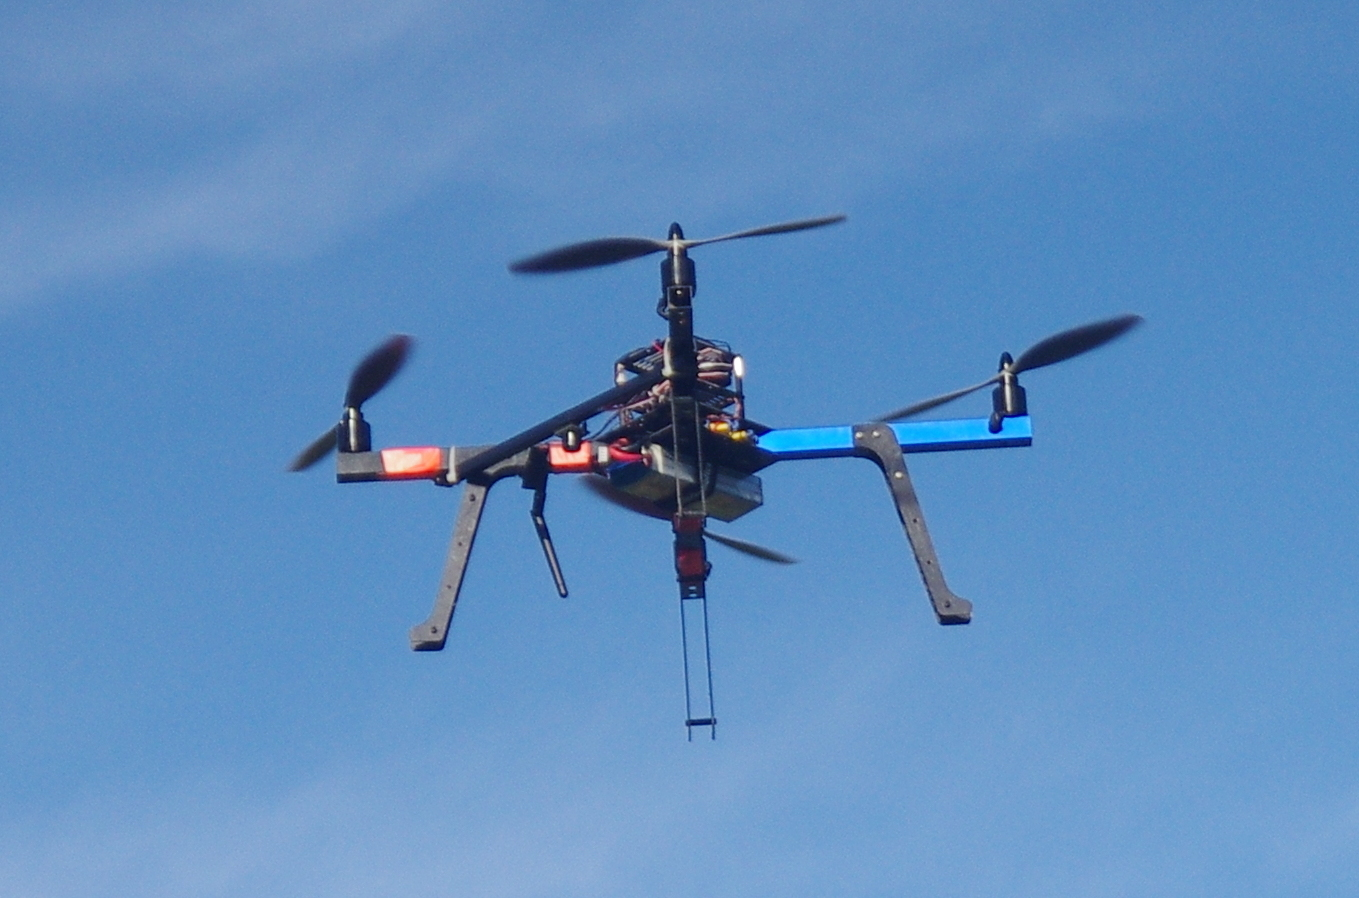
\includegraphics[width=\textwidth]{images/drone.jpg}
    \caption{Our test quadcopter in action.}
    \label{fig:drone}
\end{figure*}


\section{Prior Work}
%% CONSTANTIN
% Problem was solved in several papers in the early 21st century, using a gas powered helicopter and custom code. 

\section{Approach}

\subsection{Architecture}
%% CONSTANTIN

\begin{figure*}[h]
    \centering
    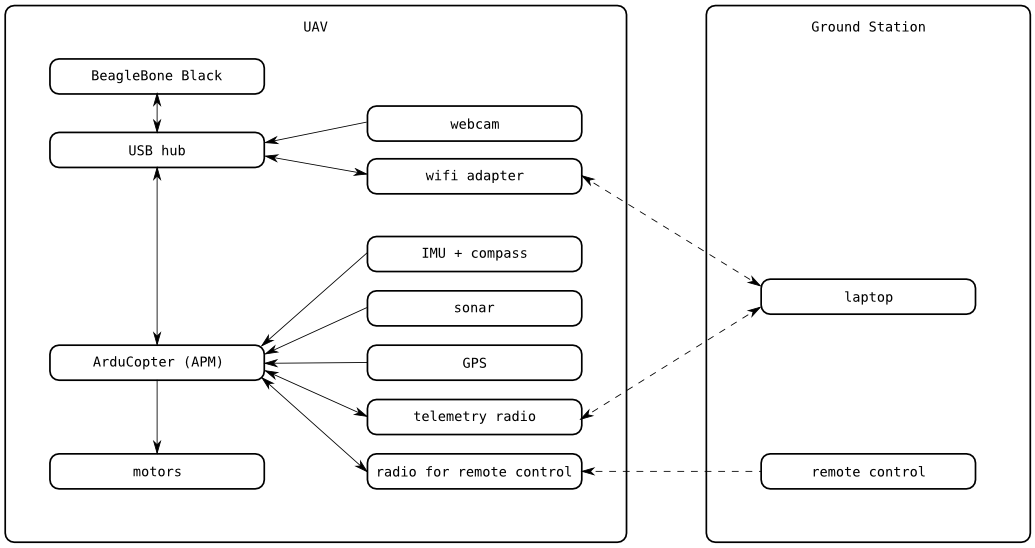
\includegraphics[width=\textwidth]{images/architecture.png}
    \caption{Architecture of our automated landing system for UAVs}
    \label{fig:architecture}
\end{figure*}

\begin{figure*}[h]
    \centering
    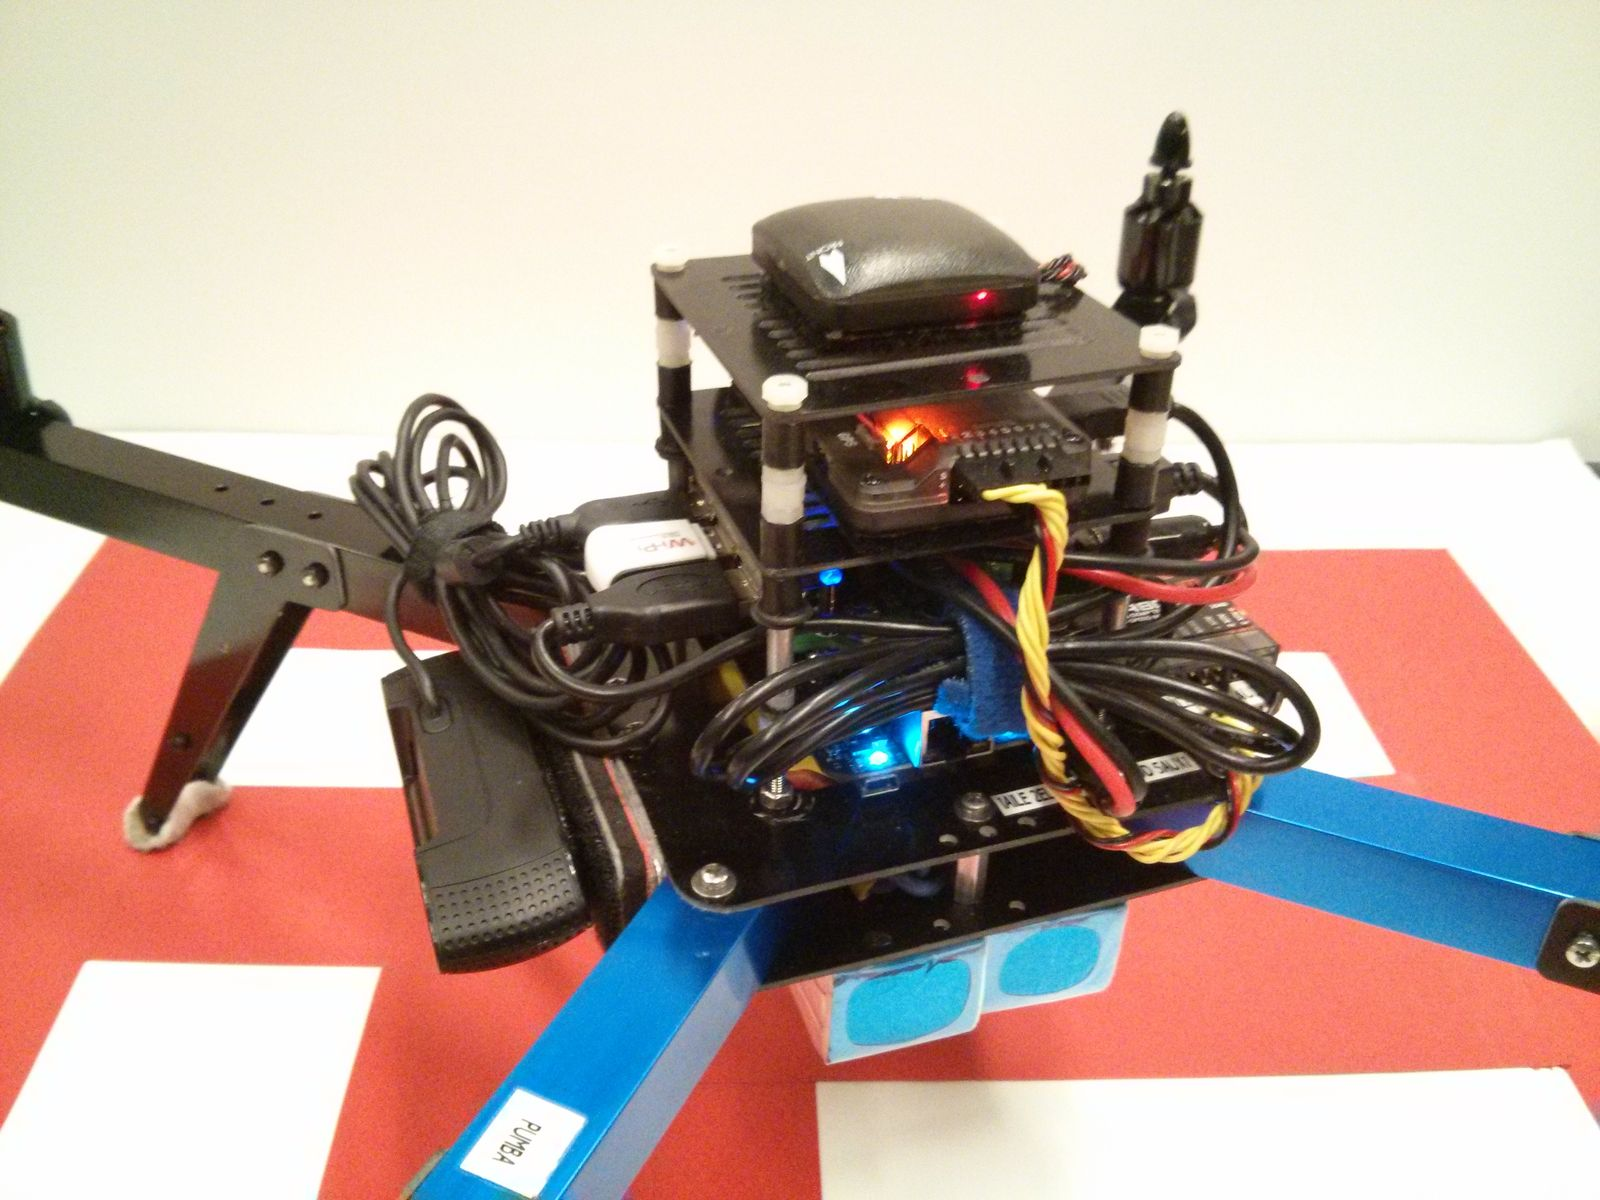
\includegraphics[width=\textwidth]{images/hardware.jpg}
    \caption{Our hardware stack installed on a quadcopter.}
    \label{fig:hardware}
\end{figure*}

% Put in weight of hardware stack and estimated power consumption?
% Estimated cost of system? Commodity hardware, etc.

% Hardware
% APM autopilot board
% BeagleBone black
% Logitech C920 Webcam (chosen for global shutter, to hopefully minimise motion blur)
% Powered USB hub
% EyePi wi-fi adaptor

% Software + Libraries Used
% ArduCopter autopilot software
% ROS
% Arm HF Linux
% roscopter library
% OpenCV

\subsection{Vision}
%% NAHUSH 
% Describe the vision approach we took

\subsubsection{Corner Detection}
%% NAHUSH

\begin{figure*}[h]
    \centering
    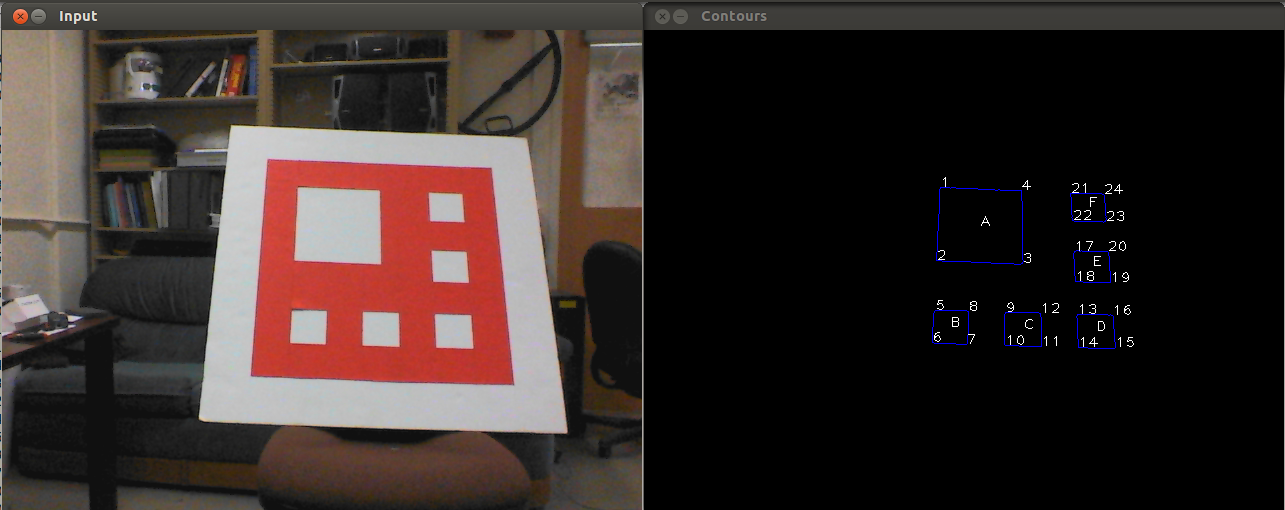
\includegraphics[width=\textwidth]{images/corners.png}
    \caption{Corner detection in action.}
    \label{fig:corners}
\end{figure*}

\subsubsection{Pose Estimation}
%% CONSTANTIN

Input: 24 point correspondences
Output: camera pose (x, y, z, roll, pitch, yaw)
Have 48 equations (2 for each point pair)
System of equations has 6 degrees of freedom
Solve it using an SVD trick


\subsection{Control}
%% SUNIl

% Simple Proportional controller
% Handed off real time control to 'Loiter' mode of the autopilot

% State estimates from barometric pressure and pose estimation

\begin{figure*}[h]
    \centering
    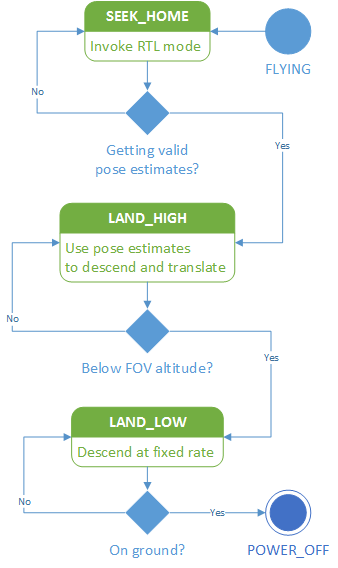
\includegraphics{images/statediagram.png}
    \caption{The state diagram of our landing controller.}
    \label{fig:statediagram}
\end{figure*}

\subsection{Software Integration}
%% SUNIL

% A brief word on ROS + diagram showing the flow of messages?

\section{Results}

\subsection{Pose Estimation Accuracy}
%% CONSTANTIN

% true height	z mean	z std	x std	y std	yaw std
% 88 cm	89.3 cm	0.05 cm	0.43 cm	0.39 cm	0.12 °
% 120 cm	121.1 cm	0.08 cm	1.16 cm	1.06 cm	0.12 °
% 170 cm	172.0 cm	0.18 cm	2.74 cm	2.17 cm	0.07 °
% 226 cm	229.0 cm	0.54 cm	6.51 cm	6.05 cm	0.34 °


\subsection{Performance}
%% CONSTANTIN

Camera is capable of 30 FPS
Just capturing frames: 11.2 FPS
Pose estimator running: 3.0 FPS
Pose estimator and roscopter running: 1.6 FPS

% Rate our system against the system they had in 2001 which ran at near real time FPS

\subsection{Control}
%% SUNIL 
% How did our controller do?
% Field of view of camera and size of landing pad meant no accurate Z estimates
% below ~ 2m.
% Noisy sensor data = state transitions wer edifficult

\section{Challenges}
One of the significant impediments to our project was integrating working hardware. In this section, we describe the issues we had and how they might be mitigated in the future.

\subsection{Integration of Hardware}
%% CONSTANTIN
% A brief note on the hardware travails we had.

\subsection{Image Quality}
%% NAHUSH
% Mention the issue with motion blur up in the air and possible solutions (better camera with more fine grained control)

\begin{figure*}[h]
    \centering
    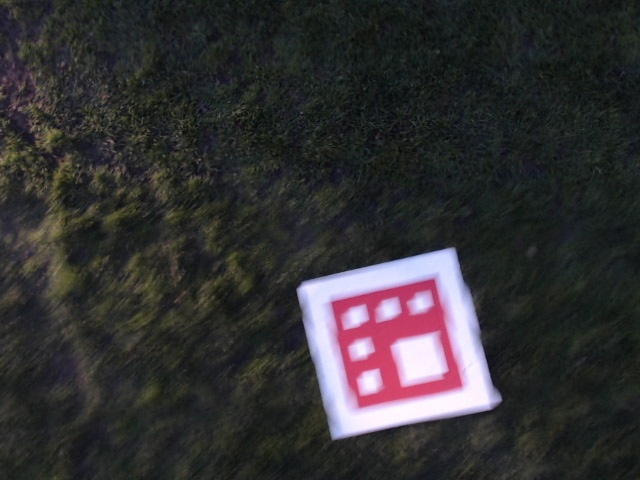
\includegraphics[width=\textwidth]{images/badimage.jpg}
    \caption{An example of a bad image.}
    \label{fig:badimage}
\end{figure*}

\subsection{Field of View}
%% NAHUSH

% Drone needs to be at 1 metre to see the landing pad.
% Practically, this means we need to be at about 2 metres to get
% pose estimates.

% height	visible land area
% 1 m	1.37 m x 0.77 m
% 2 m	2.75 m x 1.54 m
% 4 m	5.50 m x 3.07 m
% 8 m	11.0 m x 6.14 m
% 16 m	22.0 m x 12.3 m

\begin{figure*}[h]
    \centering
    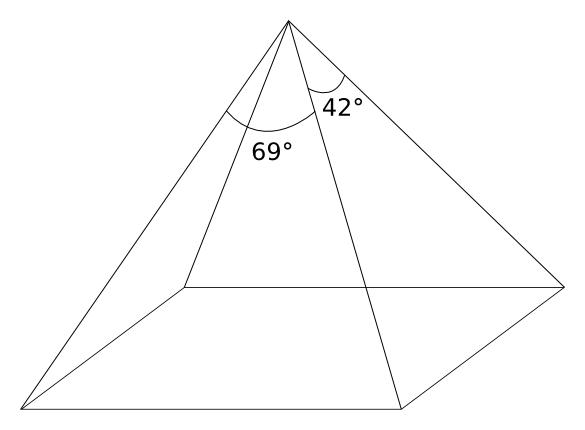
\includegraphics[width=\textwidth]{images/fov.png}
    \caption{Field of view of our webcam.}
    \label{fig:fov}
\end{figure*}

\subsection{Weather}
%% SUNIL

% Loiter mode works well with little wind but struggles when there is heavy wind
% This means that our landing controller oscillates wildly.

\section{Conclusion \& Future Directions}

Use higher quality optics.
Explore landing pad design.
Allow landing in darker scenarios.
Use more advanced control loops (PID instead of just P).
Rewrite roscopter in C++.
Integrate sonar sensor for more accurate altitude estimates.

\end{document}
